\documentclass[useAMS,usenatbib]{mn2e}
\usepackage{myaasmacros}
\usepackage{graphicx}
\usepackage{ulem}
\usepackage{color}
\usepackage{amsmath}

% Some definitions of things I always use here:
\def\ltsima{$\; \buildrel < \over \sim \;$}
\def\simlt{\lower.5ex\hbox{\ltsima}}   
\def\gtsima{$\; \buildrel > \over \sim \;$}
\def\simgt{\lower.5ex\hbox{\gtsima}}
\def\siglos{\sigma_{\text{LOS}}}
\def\siglosi{\sigma_{\text{LOS},i}}
\newcommand\bcite[1]{(\citeauthor{#1} \citeyear{#1})}

\newcommand{\changefont}[3]{
\fontfamily{#1} \fontseries{#2} \fontshape{#3} \selectfont}

\newcommand{\TODO}[1]{\textsc{\textbf{\textcolor{red}{(TODO: #1)}}}}

% Some definitions for the priors:
\def\gprior{{\tt gprior}}
\def\cprior{{\tt cprior}}
\def\bprior{{\tt bprior}}
\def\lbprior{{\tt lbprior}}

%Some definitions for rhodm etc:
\def\vztwo{\overline{v_z^2}}
\def\vztwoi{\overline{v_{z,i}^2}}
\def\rhodisc{\rho_\mathrm{disc}(z)}
\def\rhodmext{\rho_\mathrm{dm,ext}}
\def\rhodm{\rho_\mathrm{dm}}
\def\rhoeff{\rho_\mathrm{dm}^\mathrm{eff}}
\def\nuobs{\nu_\mathrm{obs}(z)}

\title[A non-parametric method for mass modelling spherical systems]{A non-parametric method for mass modelling spherical systems}

\author[Steger]{P. Steger$^1$\thanks{E-mail: psteger@phys.ethz.ch}, D. von Rickenbach$^1$, J. I. Read$^{1,2}$\\
$^1$Institute for Astronomy, Department of Physics, ETH Z\"urich, Wolfgang-Pauli-Strasse 27, CH-8093 Z\"urich, Switzerland\\
$^2$Department of Physics, University of Surrey, Guildford, GU2 7XH, UK
}

\begin{document}

\maketitle

\begin{abstract}
We propose a new non-parametric method to determine the mass
distribution in spherical systems. A high dimensional parameter space
encoding tracer density, line of sight velocity dispersion and total
mass density is sampled with an Monte Carlo Markov Chain.

Without assumptions on the functional form of any of these profiles,
we can reproduce liably the total mass density of mock dwarf galaxies,
and disentangle the degeneracy between dark matter density and tracer
velocity anisotropy.

We show early applications to observed dwarf galaxies, and point out
what data quality is required to yield a sensible estimate.
\end{abstract}

\begin{keywords} galaxies: dwarf  -- galaxies: fundamental parameters  -- galaxies: kinematics and dynamics -- cosmology: dark matter
\end{keywords}

% input does not clear page, include does. could use newclude package and include*

\section{Introduction}\label{sec:introduction}


%%% Local Variables:
%%% mode: latex
%%% TeX-master: "Steger+_2014_OtherDwarfs"
%%% End:


%\TODO{input method, test, results, conclusions, acks}
\section{Method}\label{sec:method}

The collisionless Boltzmann equation for a spherical system with
gravitational potential $\Phi$,

\begin{equation}
\frac{\text{d}f}{\text{d}t} = \frac{\partial f}{\partial t} + \nabla_{\vec{x}} f\cdot\vec{v} - \nabla_{\vec{v}} f\cdot\nabla_{\vec{x}}\Phi = 0,
\end{equation}

describes the motion of tracer stars with distribution function
$f(\vec{x},\vec{v}\,)$.


In spherical coordinates $(r, \theta, \phi)$, the collisionless
Boltzmann equation then reads as

\begin{equation}
\frac{\partial f}{\partial t} + \dot{r}\frac{\partial f}{\partial r} + \dot{\theta}\frac{\partial f}{\partial \theta} + \dot{\phi}\frac{\partial f}{\partial \phi} + \dot{v}_r\frac{\partial f}{\partial v_r}+\dot{v}_\theta\frac{\partial f}{\partial v_\theta} +\dot{v}_\phi\frac{\partial f}{\partial v_\phi} = 0
\end{equation}

with velocities

\begin{eqnarray}
\dot{r}       &=& v_r,\\
\dot{\theta}  &=& v_\theta/r\\
\dot{\phi}    &=& v_\phi / r \sin\theta.
\end{eqnarray}

The assumption of steady state hydrodynamic equilibrium gives
$\partial f/\partial t=0$ and $\bar{v}_r=0$, and using spherical
symmetry $\bar{v}_\theta=0$, $\bar{v}_\phi=0$, with a unique
tangential velocity dispersion
$\sigma_\phi^2=\sigma_\theta^2=\sigma_t^2$ and a fourth order moment $\bar{v_r^4}$ we get

\begin{eqnarray}\label{eq:Jeans}
\frac{1}{\nu}\frac{\partial}{\partial r}(\nu\sigma_{r}^2) + 2\frac{\sigma_{r}^2-\sigma_{t}^2}{r} &=& -\frac{\partial \Phi}{\partial r} = -\frac{GM(<r)}{r^2},\\
\frac{\partial}{\partial r}(\nu\bar{v_r^4})+\frac{2\beta}{r}\nu\bar{v_r^4}+3\nu\sigma_r^2\frac{\partial\Phi}{\partial r}&=&0,
\end{eqnarray}

with enclosed mass $M(<r)$, gravitational constant $G =
6.67398\cdot10^{-11} \text{m}^3/\text{kg}\,\text{s}^2$. The departure
from spherical hydrostatic equilibrium $\sigma_r^2=\sigma_t^2$ is
measured by the anisotropy parameter

\begin{equation}
\beta \equiv 1-\frac{\sigma_t^2}{\sigma_r^2}
\end{equation}

with values in the range from $-\infty$ (purely circular orbits)
through $0$ (hydrostatic equilibrium) to $1$ (purely radial orbits).

Integrating both sides of equation \ref{eq:Jeans} gives the main
equation of this paper,

\begin{equation}\label{eq:main}
\sigma_r^2(R) = \frac{1}{\nu(R)}\exp\left(-2\int_{r_{min}}^{R}\frac{\beta(s)}{s}\text{d}s\right)\cdot\qquad
\end{equation}
\begin{equation*}
\qquad\int_R^\infty \frac{GM(r)\nu(r)}{r^2} \exp\left(2\int_{r_{min}}^r\frac{\beta(s)}{s}\text{d}s\right)\text{d}r.
\end{equation*}
\begin{equation*}
\bar{v_r^4}(R) = \frac{3}{\nu(R)}\exp\left(-2\int_{r_{min}}^{R}\frac{\beta(s)}{s}\text{d}s\right)\cdot\qquad
\end{equation*}
\begin{equation*}
\qquad\int_R^\infty \frac{GM(r)\nu\sigma_r^2}{r^2} \exp\left(2\int_{r_{min}}^r\frac{\beta(s)}{s}\text{d}s\right)\text{d}r.
\end{equation*}

For distant spherical systems, only the projected velocity dispersion
$\siglos$ and the fourth order moment $\bar{v_{\rm los}^4}$ can be
measured, which in our case is given by

\begin{equation}\label{eq:LOS}
\siglos^2(R) = \frac{2}{\Sigma(R)}\int_R^\infty \left(1-\beta\frac{R^2}{r^2}\right) \frac{\nu(r)\sigma_r^2(r) r}{\sqrt{r^2-R^2}}\text{d}r,
\end{equation}
\begin{equation}\label{eq:kappa}
\bar{v_{\rm LOS}^4} = \frac{2}{\Sigma(R)}\int_R^\infty\frac{\nu \bar{v_r^4}r}{\sqrt{r^2-R^2}}g(r,R,\beta)\text{d}r
\end{equation}
\begin{equation*}
g(r,R,\beta) = 1-2\beta\frac{R^2}{r^2}+\frac{\beta(1+\beta)}{2}\frac{R^4}{r^4}
\end{equation*}


where $\Sigma(R)$ denotes the surface mass density at radius $R$. 

As in \cite{Lokas+2005}, we will compare the kurtosis

\begin{equation*}
\kappa_{\rm LOS}=\frac{\bar{v_{\rm LOS}^4}}{\sigma_{\rm LOS}^4}
\end{equation*}

between data and our model.

In the following, we present a non-parametric method for the solution
of equation \ref{eq:LOS} for the total gravitating mass density
$\rho(r)$, given observed tracer density profiles $\nu(r)$ and
$\siglos(r)$, where $r$ denotes the projected two-dimensional radius
from the center of mass of the spherical system. Following
\cite{Jardel+2012} we write the overall density profile $\rho(r)$ as

\begin{equation}
    \rho(r) = \frac{M_*}{L}\cdot \nu(r)+\rho_{\rm{DM}}(r)
\end{equation}

and assume constant mass-to-light ratios $M_*/L$ for the tracer
populations in our mock datasets. We are ultimately interested in
$\rho_{\rm{DM}}$, which is $\rho_{\rm{DM}}(r)\approx\rho(r)$ when
neglecting the mass of the tracer populations. This assumption is
valid for our mock data and any observed system with high dark matter
content in the center, where the tracer populations reside. We will
drop said assumption when working on real data.

We get the enclosed mass $M(<r)$ from the density via

\begin{equation}
M(<r) = \int_0^r \rho(r) r^2 \text{d}r,
\end{equation}

which shows up in eq. \ref{eq:main}. In principle, the method can be
generalized to investigate alternative gravity models, if the
acceleration $GM(r)/r^2$ is replaced with the respective form of
$-\partial\Phi/\partial r$.

The degeneracy between mass $M$ and velocity anisotropy $\beta$ is
accounted for: For any non-isothermal system, we let vary the
anisotropy $\beta(r)$ as well. We checked that in the case of a simple
Hernquist profile, $\beta(r)\approx0$ is retrieved correctly.

We sample the parameter space $[\nu_i, \siglosi, \rho]$ for distinct
populations $i=1...N$ of stellar or gaseous tracers with a Monte Carlo Markov Chain method.

Early approaches were performed with a custom MCMC method. It proved
unfeasible to sample the whole parameter space on human timescales due
to its high dimensionality.

To circumvent many likelihood evaluations around a local minimum, we
changed the underlying sampling method to use several MCMC walkers,
along the lines recently described in \citep{Nelson+2013} for their
parallel code RUN DMC to analyze radial velocity observations of
planetary systems.

A useful framework was found in MultiNest (\cite{Feroz+2009}), which
is a Bayesian nested sampling algorithm to generate posterior samples
from non-trivial distributions in high dimensions.

There are a large number of parameters from the representation of the
radial profiles of each of those in $N_{bin}$ bins, with only very few
constraints from physical priors. The functional form of the profiles
is not predescribed. This is what we call {\it non-parametric}.

MultiNest samples the $n$-dimensional hypercube $\kappa=[0,1]^n$,
which needs to be translated into physical prior distributions for
each of the parameter profiles:

The overall density $\rho$ is represented in terms of the logarithmic
density slopes $n(r_i)=\kappa_{\rho_i} = (\kappa_{\rho_i})^2$, $1\leq
i\leq N_\rho+3$ and calculated as

\begin{equation*}
    \rho(r) = \rho(r_{1/2})\cdot\exp\left[\int_{r_{1/2}}^rn(s)\text{d}s\right],
\end{equation*}

with the density at half-light radius $\rho(r_{1/2})=$, and $n(r)$
interpolated linearly in between bin radii $r_{i-1}<r<r_{i}$. We
prescribe two additional slopes $n_0 < -3, n_\infty>-3$ for the
asymptotic density slopes towards $r=0$ and $r=\infty$, which are
reached at half the smallest and twice the largest bin radius.

The velocity anisotropy $\beta$ is allowed to vary freely in the
interval $[0, \infty[$ by sampling the modified, symmetric $\beta_*$
(\TODO{cite Read}),

\begin{equation*}
    \beta_* = \frac{\sigma_r^2-\sigma_t^2}{\sigma_r^2+\sigma_t^2} = \frac{\beta}{2-\beta} \in [-1,1]
\end{equation*}

with a polynomial s.t.

\begin{equation*}
    \beta_*(r) = \sum_i=0^{N_\beta} \kappa_{\beta_i}\cdot\left(\frac{r_i}{r_{\text{max}}}\right)^i,
\end{equation*}

where $\kappa_{\beta_i}\in [0,1]$. With this method, unphysical
$\beta>1$ are possible, which we prevent with a correction

\begin{equation*}
    \beta_*(r_i) := \min(\max(\beta_*(r_i), -1),1).
\end{equation*}

This approach allows us to change the number of parameters $N_\beta$
easily, and to sample many qualitatively different models --
isotropic, radially biased, tangentially biased, and any gentle
transitions between those -- with very few parameters.

In a next step, $\siglosi(r)$ is calculated from $\nu(r)$, $\rho(r)$,
and $\beta(r)$ according eq. \ref{eq:LOS}. This is done numerically,
involving three integrations, which are performed with polynomial
extrapolations of the integrands up to infinity, s.t. missing
contributions from $r>r_{max}$ do not lead to an artificial falloff of
$\siglos$. The additional parameters of the slopes are calculated from
the values at lower radii, thus preventing the introduction of any
further parameters.

The last step involves comparison of the projected $\nu_i(r)$,
$\sigma_i(r)$ and $\beta_i(r)$, if available, to the data for the
tracer populations to get a likelihood based on the overall
goodness of fit

\begin{eqnarray}
\chi^2 &=& \sum_{i=1}^N \chi_{\nu,i}^2 + \chi_{\sigma,i}^2 + \chi_{\beta,i}^2\\
\chi_{\nu,i}^2 &=& \sum_{j=1}^{N_{bin}} \left(\frac{\nu_{i,\text{data}}(r_j)-\nu_{i,\text{model}}(r_j)}{\epsilon_\nu(r_j)}\right)^2.
\end{eqnarray}

and accordingly for $\chi_{\sigma,i}^2$ and $\chi_{\beta,i}^2$. In
absence of a measured $\beta_i(r)$, we set $\chi_{\beta,i}^2=0$.

\subsection{Binning characteristics}

The number of bins for $\rho, \nu_i, \beta_i$, and $\sigma_i$ are free
parameters. They are set to fulfill

\begin{equation}
n_\nu = n_\sigma = n_\beta = n_\rho \leq n_{\text{data}}
\end{equation}

with number of datapoints $n_{\text{data}}$. This choice simplifies
integration greatly, and prevents invention of information on scales
smaller than the frequency of datapoints.

\TODO{check that nbin is set s.t.}

\begin{equation}
\chi^2_{red} = \frac{\chi^2}{n_{\text{data}} - n_\nu - n_\sigma - n_\beta - n_\rho -1}
\end{equation}

is minimized, and still the whole parameter space is tracked.

The whole parameter space for $\beta_i$ is sampled with $n_\beta=12$
if $n_{\text{data}}=30$ in the case of 10000 tracers.

The dark matter density is calculated by subtracting the measured
baryon density from the dynamical mass density.

\subsection{Priors}
Following priors are included in the model, and help to reject
unphysical samplings from the start:

\begin{enumerate}
    \item[1)] baryon prior: $\rho(r) \geq
    \rho_b(r)-\epsilon_{\rho,b}(r) \forall r\geq0$, ensures that no
    models with overall densities below the measured baryon density
    are considered any further;

\item[2)] mass restriction: $M(r>r_{max}) \leq M(<r_{max})/3.$, rejects any
  model which has more than $M_\infty/3$ in the extrapolated bins;

\item[3)] $\beta_i(r+\Delta r)-\beta_i(r) < 0.5$: prevent any sudden
  jumps in $\beta_i$;
\end{enumerate}

We show in the appendix what effects the disabling of these priors
have.

\subsection{Splitting by metallicities}\label{sec:metals}

Observations of the abundances of metals and chemical species in the
stellar atmospheres show that the ensemble of stars in a dwarf galaxy
or globular cluster can be split into populations.

The first approach by \cite{WalkerPenarrubia2012} showed that if the
population of e.g. Fornax is split into two populations, and each of
their half-light radius and mass are determined, restrictions on the
overall potential can be drawn. Using this approach, they prefer a
cored DM profile for Fornax.

In our test suite there are dwarf galaxies with different scale radii
and small differences in the mean of the metallicity for the two
populations of stars. In order to reproduce the underlying populations
we use an inset MCMC with assumptions that

\begin{enumerate}
\item Foreground stars are younger than most of the dSph member
  stars. Therefore, they show a high metallicity and can be removed
  from the dataset with a single cut in metallicity;
\item the remaining stellar components are divided into two
  populations;
\item the fraction of stars in population 1 is sampled in a uniform
  way in the range $[0.2,0.8]$;
\item both populations show a normal distribution in metallicity with
  the same width;
\item the initial values of the means are set to half and twice the
  mean metallicity, to allow for a reasonable difference between the
  means. This difference is then subsequently sampled assuming a
  normal distribution;
\item 2000 iterations for burn-in and 1000 iterations for subsequent
  parameter estimates are used, with a thinning by factor 10 to reduce
  correlations between subsequent models. This procedure converges in
  all tested cases.
\end{enumerate}


To test whether the assignment into populations is a valid one, we
want to check whether the population is in equilibrium with the
overall potential.

\begin{figure*}
\begin{center}
\hspace{-7mm}
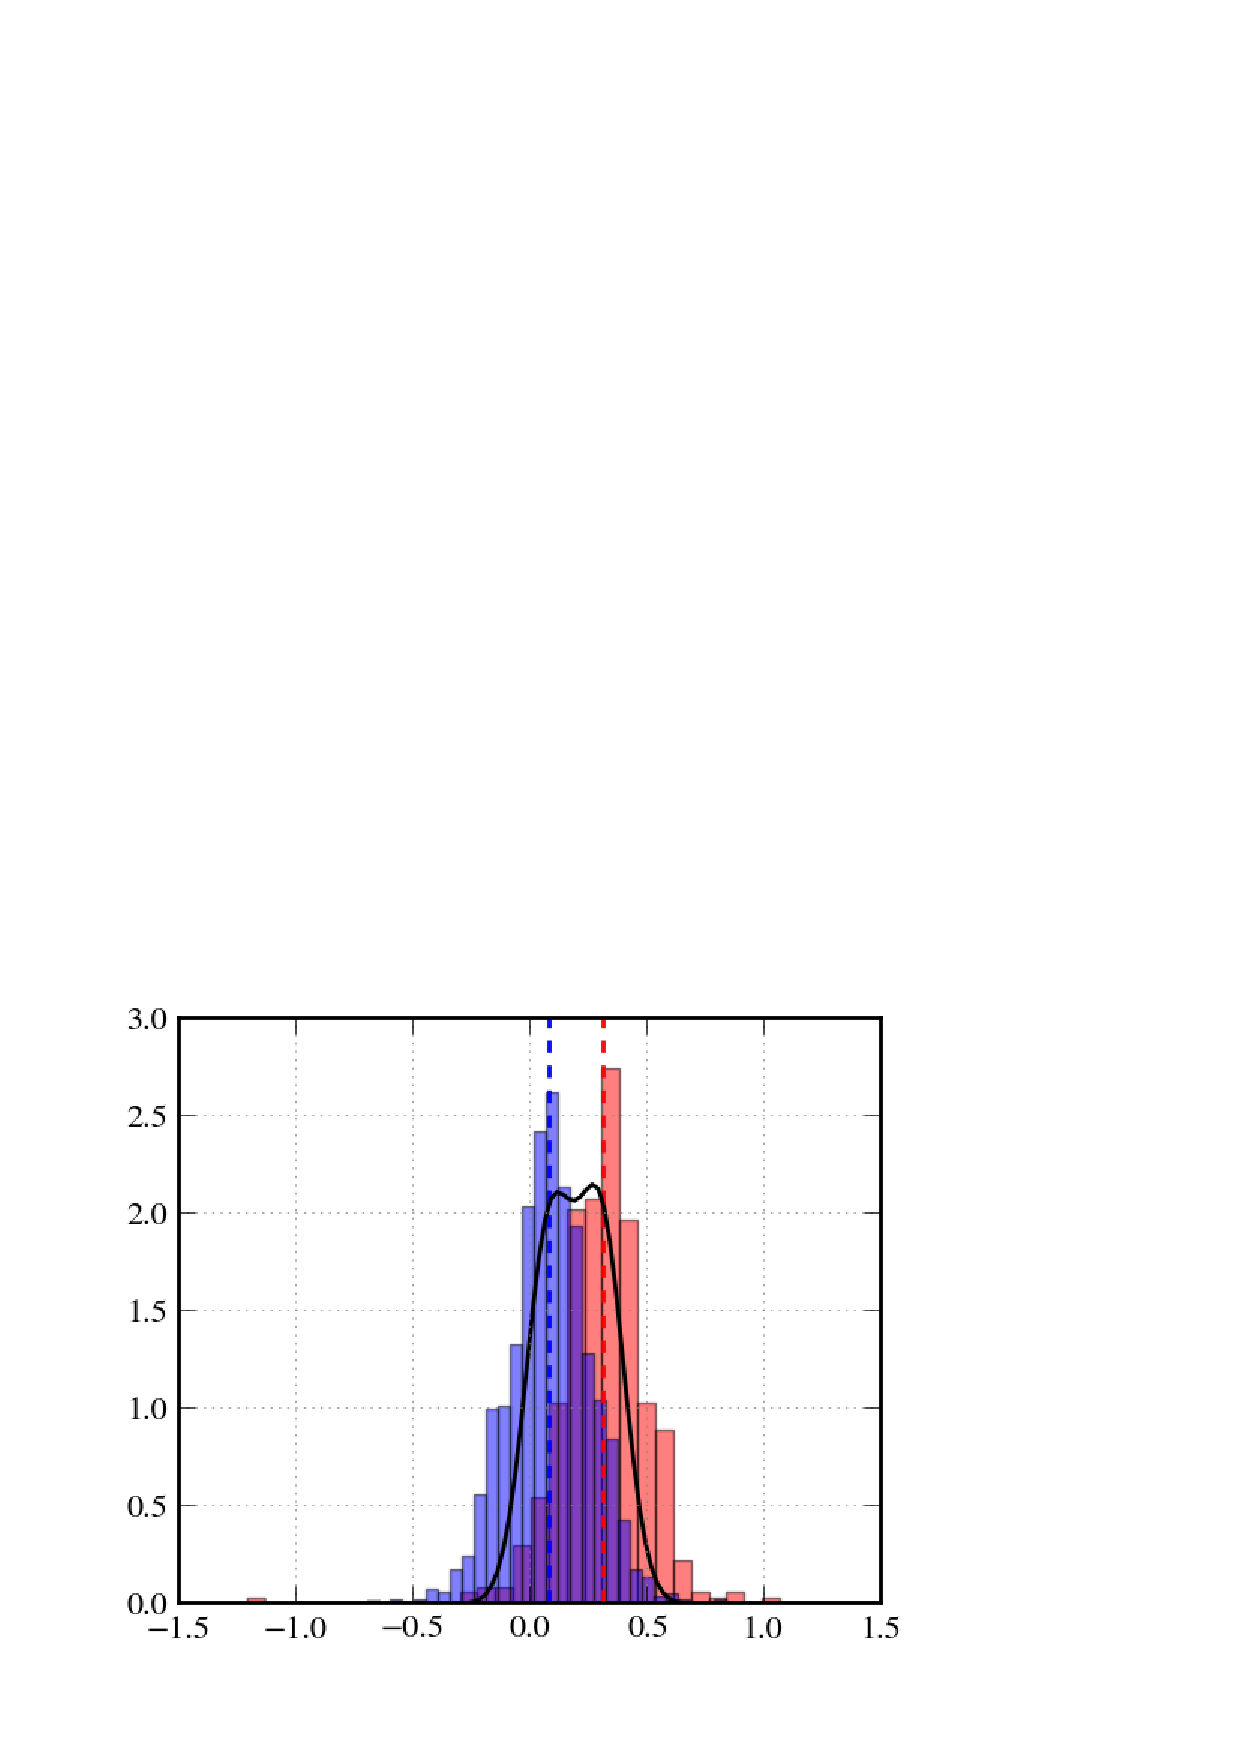
\includegraphics[width=0.5\textwidth]{fig/pymcmetals.png}
\caption{Distribution function of two populations (filled histograms) and the reproduced overall distribution.}
\label{fig:pops}
\end{center}
\end{figure*}

The routine then assigns each particle to one of the two populations,
based on its Mg metallicity. The procedure assigns $75\pm4\%$ of all
stars to the correct underlying distribution. This in turn changes the
half-light radius by $110$pc and $-62$pc for initial 390 pc, 730 pc
half light radii. These changes are rather high, but the two
populations still show distinct half-light radii.

%\section{Tests}\label{sec:tests}

\subsection{Hernquist model}
To check the correct function of the integration routine, we used the
analytic formulas from \cite{Hernquist1990}:

\begin{eqnarray}
M(r) &=& M\frac{r^2}{(r+a)^2}\\
\nu(r) &=& \frac{M}{2\pi}\frac{a}{r}\frac{1}{(r+a)^3}\\
\beta(r) &=& 0
\end{eqnarray}

with mass scale $M$ and length scale $a$ as inputs, and calculated
$\siglos(r)$ with our numerical routine, including three
integrations. Working with extrapolations to the first bin turns out
to give the most stable results, corresponding nicely to the analytic
value \bcite{BaesDejonghe2002} of

\begin{eqnarray*}
\siglos(r) &=& \frac{1}{I(r)}\frac{1}{24\pi(1-r^2)^3}\times\\
           && \qquad [3r^2(20-35r^2+28r^4-8r^6)X(r) \\
           && \qquad + (6-65r^2+68r^4-24r^6)]-\frac{r}{2},\\
\sigma_r(r) &=& r(1+r)^3 \ln\left(\frac{1+r}{r}\right)\\
 &&\qquad-\frac{r(25+52r+42r^2+12r^3)}{12(1+r)},\\
I(r) &=& \frac{1}{2\pi}\frac{(2+r^2)X(r)-3}{(1-r^2)^2},\\
X(r) &=& \begin{cases}(1-r^2)^{-1/2} \text{arcsech}\,r,& \text{for}\,0\leq r\leq 1,\\
                (r^2-1)^{-1/2} \text{arcsecans}\,r,& \text{for}\,1\leq r\leq\infty
                \end{cases}.
\end{eqnarray*}



A single component model is set up according a simple Dehnen split
power-law sphere \cite{Read+2006},

\begin{equation}
\rho(r) = \frac{M_\infty(3-\gamma)}{4\pi r_S}\left(\frac{r}{r_S}\right)^{-\gamma}\left(1+\frac{r}{r_S}\right)^{4-\gamma},
\end{equation}

where $M_\infty=1$ denotes the total mass, $\gamma=1$ the logarithmic
central asymptotic slope, and $r_S=1$ the scale length. We use $10^6$
sample points, outof which $10^4$ are extracted for further analysis.

We then let $\nu, \rho, \beta$ vary. The MCMC correctly recovers the
underlying mass distribution.



\subsection{Data quality}
How many tracer stars are needed to determine the overall density
profile reliably? To address this question, we performed three runs
with a restricted set of tracer particles. In the first, $10^3$
particles were chosen out of the $10^6$ simulated particles. With
$10^4$ particles, the confidence intervals shrink. These $10^4$
particles are split then into two populations of each $5\cdot10^3$
particles, with different scalelengths of $r_S$ and $r_S/10$. Most of
the second population particles are inside the first two bins, so the
overall convergence is not visibly affected above the third bin.
However, the models are better constrained around the scalelengths of
both tracer populations. This is expected from
\citet{WalkerPenarrubia2011}, as any velocity anisotropy sampling
yields the same mass constraint there.


\begin{figure*}
\begin{center}
\hspace{-7mm}
\includegraphics[width=0.3\textwidth]{fig/hernquist1e3.eps}
\includegraphics[width=0.3\textwidth]{fig/hernquist1e4.eps}
\includegraphics[width=0.3\textwidth]{fig/hernquist2x5e3.eps}
\caption{Hernquist profile found by MCMC model (red) for $10^3$,
  $10^4$ and 2 times $5\cdot10^3$ tracer particles. Black curve
  shows the enclosed mass derived from model.}
\label{fig:hernquist1e3}
\end{center}
\end{figure*}


 % Hernquist tests no more required
\section{Results}\label{sec:results}

We apply our method to another set of mock data, the spherical models
for the Gaia challenge by Walker and Penarrubia. They consist of
dynamical tracer populations with density distribution

\begin{equation}
\nu_*(r) = \nu_0\left(\frac{r}{r_*}\right)^{-\gamma_*} \left[1+\left(\frac{r}{r_*}\right)^{\alpha_*}\right]^{(\gamma_*-\beta_*)/\alpha_*}
\end{equation}

inside dark matter halos of the form

\begin{equation}
\rho_{\text{DM}} = \rho_0\left(\frac{r}{r_{\text{DM}}}\right)^{-\gamma_{\text{DM}}}\left[1+\left(\frac{r}{r_{\text{DM}}}\right)^{\alpha_{\text{DM}}}\right]^{(\gamma_{\text{DM}}-\beta_{\text{DM}})/\alpha_{\text{DM}}}
\end{equation}

with scale radii $r_*, r_\text{DM}$, inner and outer logarithmic
slopes of $\gamma_*, \gamma_{\text{DM}}$ and
$\beta_*,\beta_{\text{DM}}$, with transition parameters $\alpha_*,
\alpha_{\text{DM}}$.

The anisotropy follows the functional form of \citet{Osipkov1979} and
\citet{Merritt1985},

\begin{equation}
\beta_{\text{anisotropy}}(r)=1-\frac{\sigma_\theta^2}{\sigma_r^2} = \frac{r^2}{r^2+r_a^2}.
\end{equation}

with scale radius $r_a$, turning over from nearly isotropic at $r\to
0$ to radially isotropic at $r_*=r_a$.

Of these distributions, finite samplings are taken and converted to
mock observational data including spectral indices, systemic
velocities, proper motions, binary motion.


\subsection{Cusps and Cores}

Applied on a profile with a core in the DM density profile, our method
converges fast in the beginning, see fig. \ref{fig:cusp}.

\begin{figure*}
\begin{center}
\hspace{-7mm}
%\includegraphics[width=0.5\textwidth]{fig/1000its.pdf}
\includegraphics[width=0.5\textwidth]{fig/recent_50k.pdf}
\caption{Reconstructed mass of a cusped model (red shows median,
  shaded areas are 68 and 90 percentiles) for $10^4$ tracer particles,
  after 50000 iterations. The black dashed curve shows the underlying
  theoretical model.}
\label{fig:cusp}
\end{center}
\end{figure*}

If run for 50000 iterations, the profile in the right plot emerges,
with broader errorbars and a slight mismatch above $r_{vir}=1000{\rm
  pc}$.

The model is best constrained around $r=500$pc, which corresponds to
the scale radius of both the stellar tracers.

For a cored profile, we have a similar result, see fig. \ref{fig:core}.

\begin{figure*}
\begin{center}
\hspace{-7mm}
%\includegraphics[width=0.5\textwidth]{fig/core_2k.pdf}
\includegraphics[width=0.5\textwidth]{fig/core_30k.pdf}
\caption{A cored profile: Reconstructed mass of the MCMC model (red
  shows median, shaded areas are 68 and 90 percentiles) for $10^4$
  tracer particles after 30000 iterations. The black dashed curve
  shows the underlying theoretical model.}
\label{fig:core}
\end{center}
\end{figure*}

Best restrictions are around $500$pc again, only this time a little
too low.

\section{Conclusions}\label{sec:conclusions}

The new non-parametric method samples the profiles of the overall
density bin-wise, and was shown to reconstruct the density of diverse
mock data.


%%% Local Variables:
%%% mode: latex
%%% TeX-master: "Steger+_2014_Fornax"
%%% End:

\section{Acknowledgements}
JIR would like to acknowledge support from SNF grant PP00P2\_128540/1.


\bibliographystyle{mn2e}
\bibliography{main}

%\TODO{include appendix}
\section{Appendix}

\subsection{Effect of Wrong Assignment of Populations}
We quantify the influence of assigning stars the wrong population by
looking at the changes for

\begin{enumerate}
\item assigning stars randomly to two population
\item assigning stars to populations based on position information
  only
\end{enumerate}

\TODO{result}

\subsection{Priors in use}
We use the priors outlined in \citep{Steger+2014}, with numerical
values in table \ref{tab:priors}:

\begin{enumerate}
  \item $\beta^*(r)$ is given in the form
    \begin{equation}\label{eqn:betastar}
      \beta^* = \frac{\sigma_r^2-\sigma_t^2}{\sigma_r^2+\sigma_t^2} = \frac{\beta}{2-\beta} \in [-1,1]
    \end{equation}
    with the following function:

    \begin{eqnarray} \label{eqn:nonparabetstar}
      \beta^*(r) &=& \frac{a_0-a_\infty}{1+\kappa \exp(\alpha\ln(r/r_s))}+a_\infty\\
      \kappa &=& \frac{a_0-a_\infty}{\beta^*(r_s)-a_\infty}-1
    \end{eqnarray}


  \item $n(r)=-{\rm d}\ln\rho(r)/{\rm d}\ln r$ is calculated by integrating its
    derivative $dn(r)/d\ln r$ -- which is given at discrete bin
    centers, and drawn from a Gaussian prior of width $\sigma$ -- with
    the additional constraint that $n(r)\geq0$. The density profile

    \begin{equation*}
      \rho(r) = \rho_{1/2}\cdot\exp\left[-\int_{\ln r_{1/2}}^{\ln r}n(s)\text{d}s\right],
    \end{equation*}

    is thus represented by its second derivatives. This enforces a
    monotonically decreasing $\rho(r)$, and further circumvents strong
    oscillations from numerical effects.

  \item no use of fourth order moments $\kappa$
  \item no use of virial parameters $\zeta_A, \zeta_B$
\end{enumerate}



\begin{table}
  \label{tab:priors}
  \caption{Priors for the \GravImage method used on Fornax.}
  \centering
  \begin{tabular}{lllll}
    Quantity & type & characteristics \\
    \hline
    $N_{bin}$ & fixed & 12\\
    $n_\beta$ & fixed & 4\\
    $dn(r)/d\ln r$ & Gaussian & mean 0, width $\sigma=5$\\
    $n(r)$ & bound & $\min(n(r))=0$\\
    $\ln \rho(r_{1/2})$ & flat & center $-1$, width $2.5$ dex\\
    $M/L$ & flat & $[0.8, 3]$
  \end{tabular}
\end{table}



%%% Local Variables:
%%% mode: latex
%%% TeX-master: "Steger+_2014_Fornax"
%%% End:


\end{document}
